\subsection{\textcolor{magenta}{Préparer le laser}}
\begin{center} $\ast\ast\ast$ Si le laser est déjà en Standby, passer tout de suite à la section \ref{ssec:allumer_le_laser}. $\ast\ast\ast$ \end{center}
\begin{enumerate}
    \item Sur chaque refroidisseur (voir figure~\ref{fig:cooler}, peser sur le bouton \textit{Run/Standby}.
        \begin{figure}[H]
        \centering
        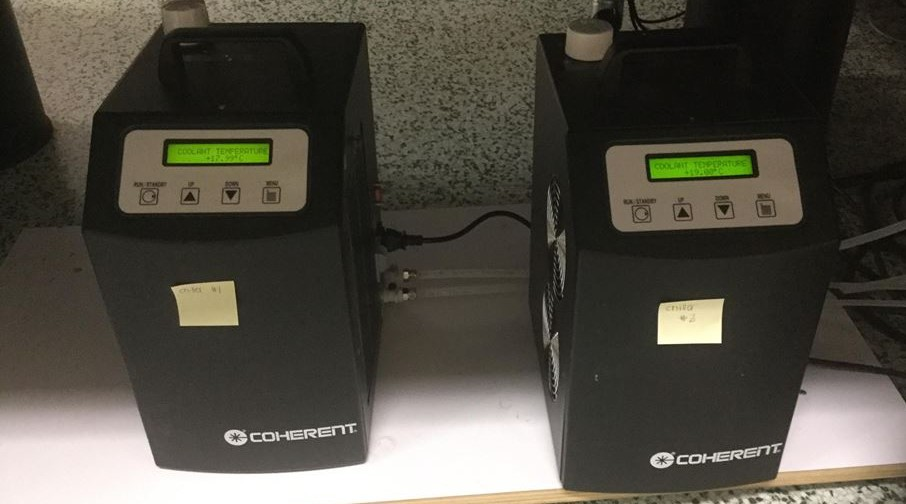
\includegraphics[width=10cm]{cooler.jpg}
        \caption{Refroidisseurs: l'un contrôle le \textit{Verdi}, l'autre le \textit{Mira} et le \textit{RegA}}
        \label{fig:cooler}
        \end{figure}
    \item Peser sur le bouton \textit{Menu}. Vérifier que \textit{Set Temperature} est à 18-19$^\circ$C.
    \item Repeser sur le bouton \textit{Menu}. Attendre que \textit{Coolant Temperature} soit à 18-19$^\circ$C (4-5 minutes).
    \item À l'arrière du \textit{contrôleur Verdi} (voir figure~\ref{fig:controleur-verdi}, mettre l'interrupteur sur \textit{On}).
        \begin{figure}[H]
        \centering
        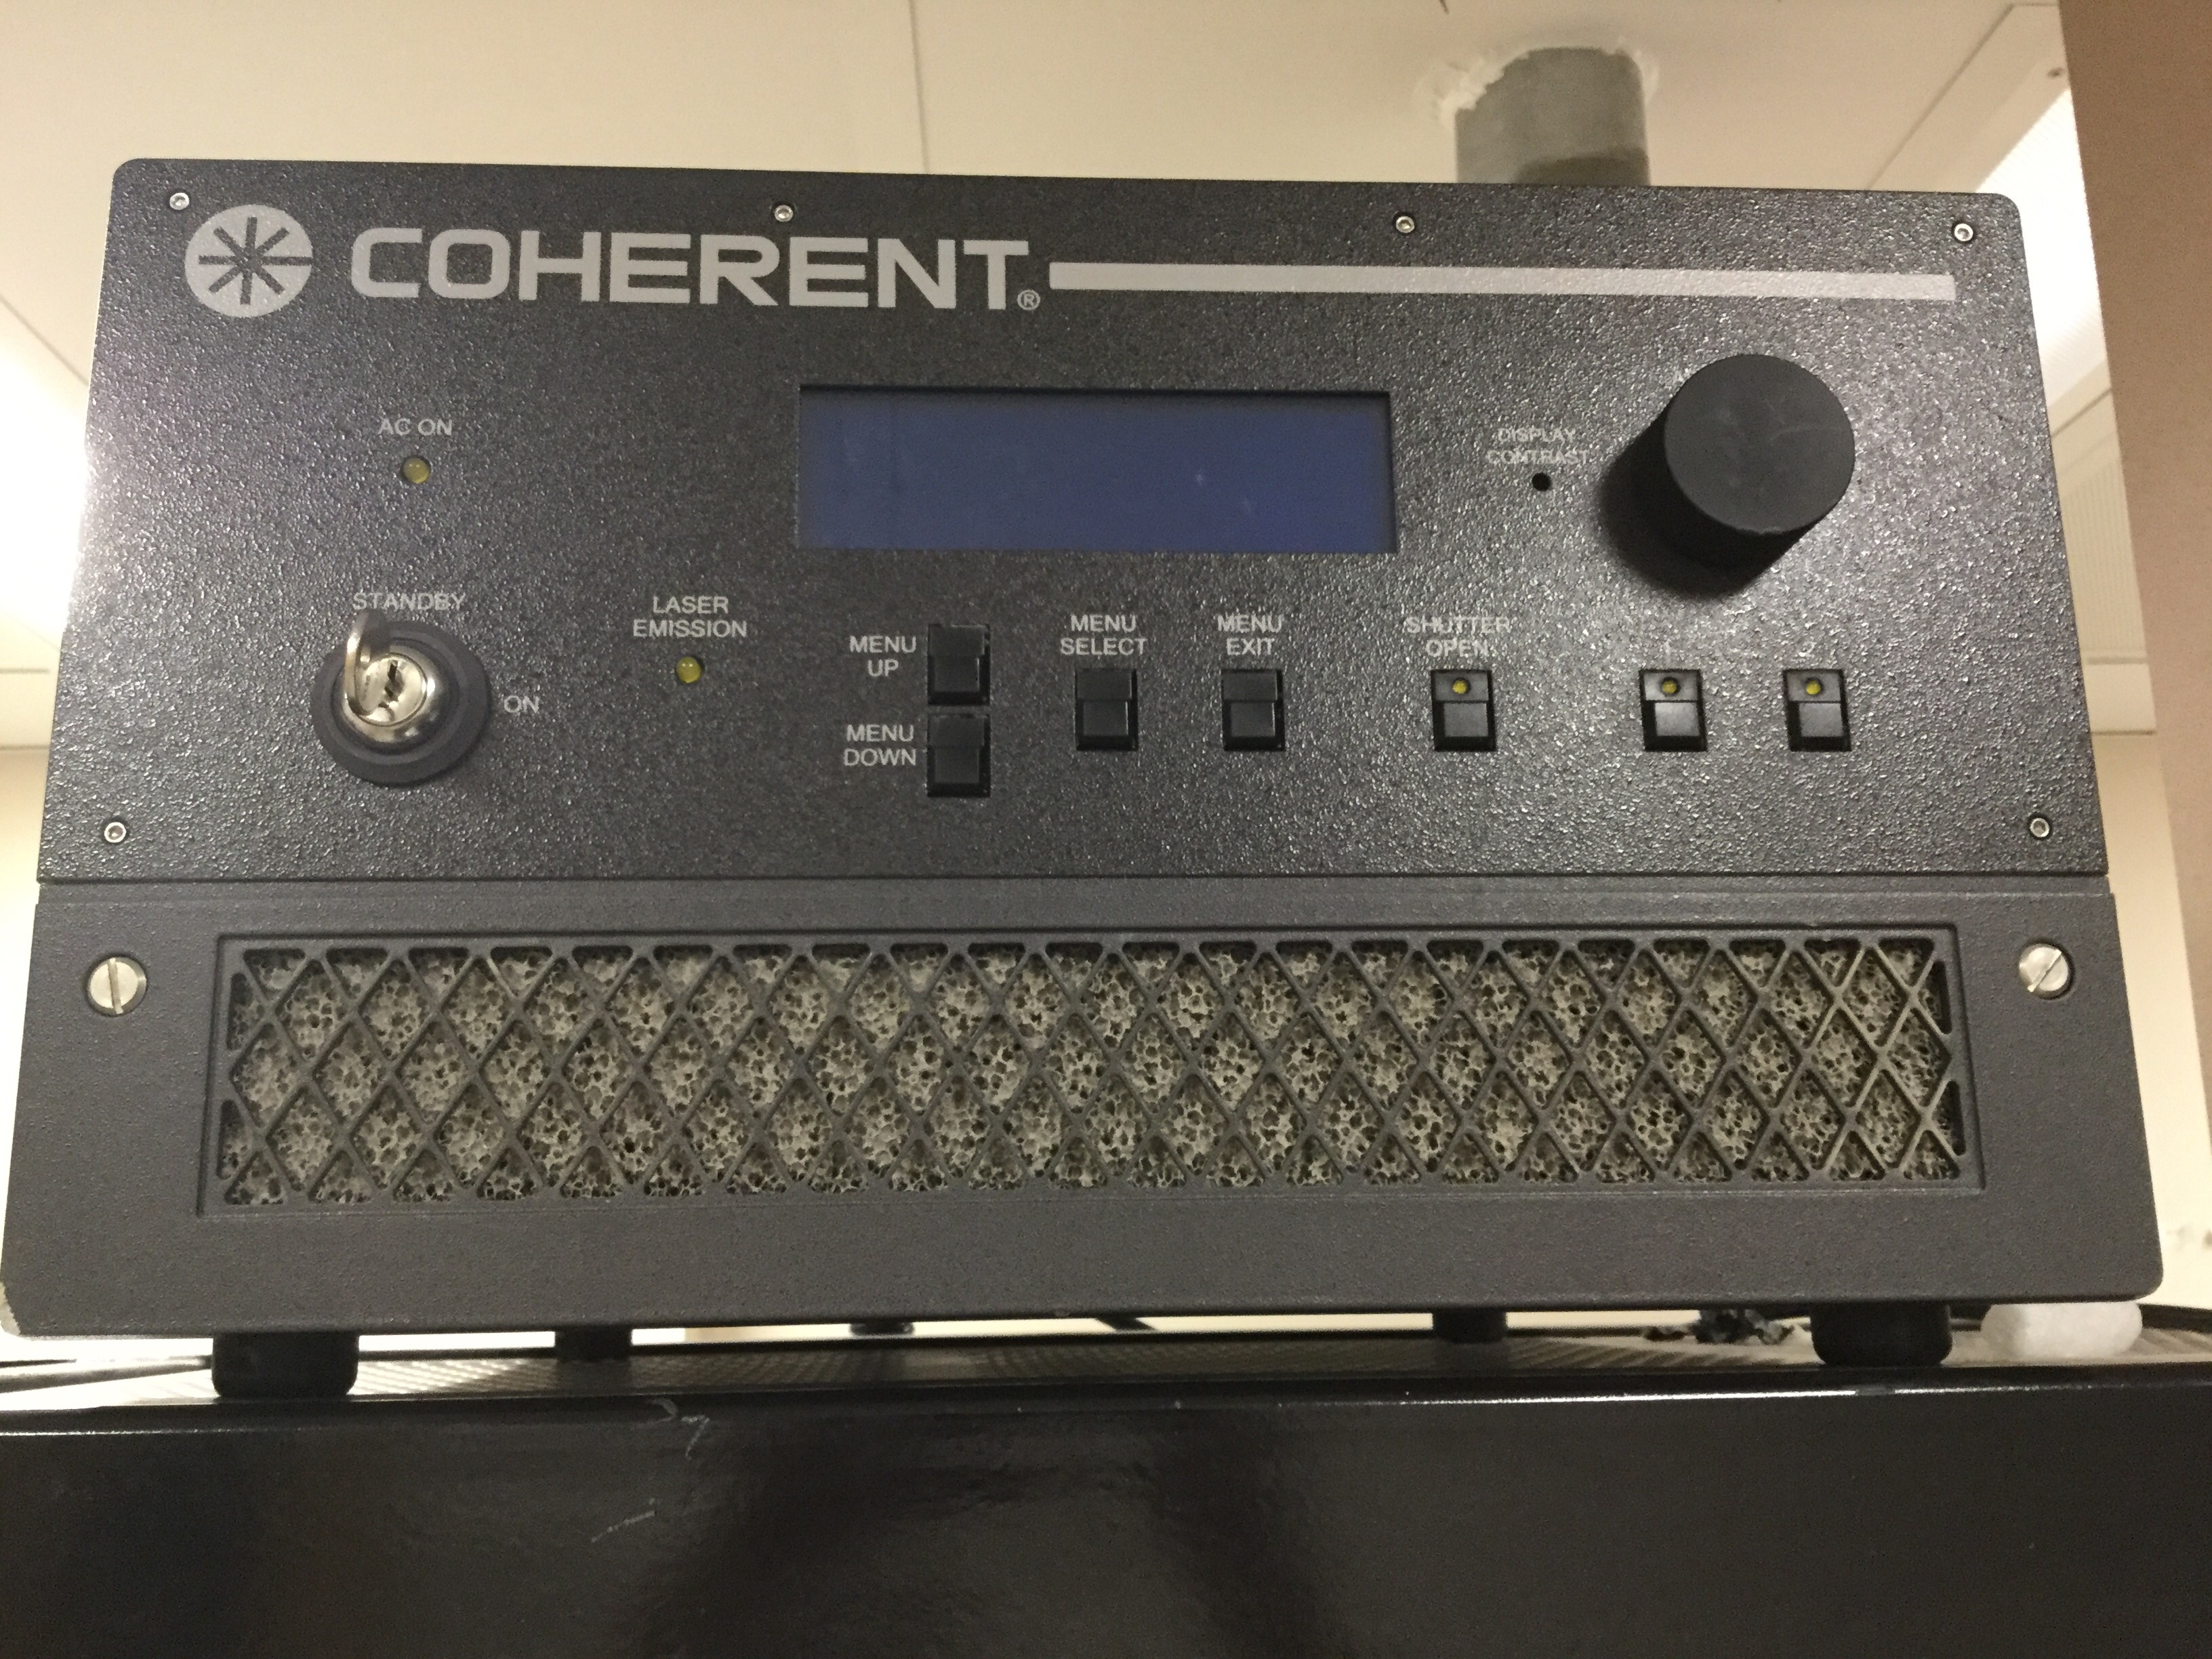
\includegraphics[width=12cm]{controleur-verdi.jpg}
        \caption{Contrôleur du \textit{Verdi}}
        \label{fig:controleur-verdi}
        \end{figure}
    \item Peser sur le bouton \textit{Menu Select}. À l'aide des boutons \textit{Menu Up} et \textit{Menu Down}, aller dans \textit{FAULT Status}. Vérifier que le message affiché est \textit{'SYSTEM OK!'}. Peser sur \textit{Menu Exit}.
    \item Aller dans \textit{LBO Settings}. Vérifier que le message affiché est \textit{'LBO Heating'}. Peser deux fois sur \textit{Menu Exit}.
    \item Vérifier que le message affiché en haut à droite est \textit{'System Warming Up'}.
    \item Tourner la roulette pour ajuster la puissance à 17~W.
    \item Attendre que \textit{'System Warming Up'} soit remplacé par \textit{'Standby'} (environ 10-15 minutes).
\end{enumerate}